% Drawing 64/07-1 -- folder 64, batch 07, archive page 122 (PDF page 123).
% Transcription: sous la première ligne, un croquis : un axe vertical et un axe horizontal se coupant à l'origine ; au-dessus, une horizontale portant les trois points marqués $\xi_1$, $\xi_3$, $\xi_2$ (de gauche à droite) ; trois droites issues de l'origine passent par ces points et sont prolongées des deux côtés.
% Kind: three lines through the origin and three marked points on a horizontal. Method 2 (schematic redraw from the facsimile). Status: ok.
% Notes: As on the page: the short vertical axis and the horizontal axis through the origin (two small ticks on the latter), the horizontal line above carrying the three marked points, labelled xi_1, xi_3, xi_2 from left to right, and the three lines through the origin and these points; the three lines and the two axes are drawn through one computed origin, each line through its marked point, produced on both sides as far as he drew them (the line of xi_1 is gone over several times on the page: drawn once). Left out: the arrow, the sign infinity and the letter t at the top left of the crop, which belong to the first line of the text. Redrawn 2026-11-12 (issue 128): to check again.
% Coordinates: 1 unit = 1 mm = 1/100 of the crop width (bbox in page fractions: [0.25, 0.115, 0.72, 0.26]).
% Redrawn by Claude (claude-fable-5-2), issue #128, 2026-11-12; not checked by a human; not compiled (no TeX in the session).
% Rights: reproduces part of the work -- behind RENDER_TRANSCRIPTS, never published by itself.
\documentclass[tikz,border=3pt]{standalone}
\usepackage{amsmath,amssymb}
\usetikzlibrary{patterns,arrows.meta}
\tikzset{pencil/.style={black!45}, struck/.style={black!35}, mpt/.style={circle,draw,inner sep=1.3pt}, pt/.style={circle,fill,inner sep=0.9pt}, opt/.style={circle,draw,fill=white,inner sep=1.1pt}}
\begin{document}
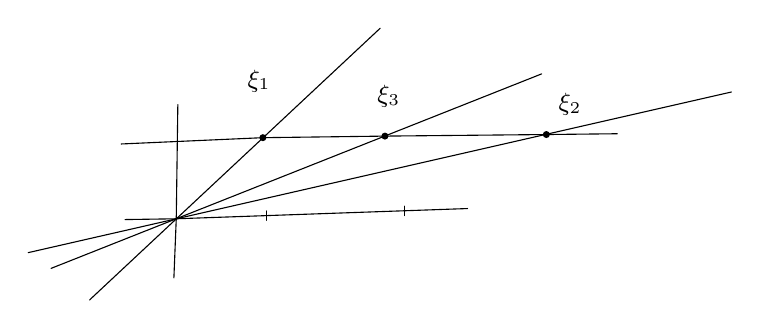
\begin{tikzpicture}[x=1mm,y=1mm,line cap=round,line join=round,font=\scriptsize]
\draw (23.7,-18) -- (23.5,-32.5) -- (23.2,-40);
\draw (17,-32.6) -- (23.5,-32.5) -- (60.5,-31.2);
\draw (35,-31.5) -- (35,-32.7);
\draw (52.5,-30.9) -- (52.5,-32.1);
\draw (16.5,-23) -- (34.5,-22.2) -- (50,-22) -- (70.5,-21.8) -- (79.5,-21.7);
\draw (12.5,-42.8) -- (49.4,-8.3);
\draw (7.6,-38.8) -- (69.9,-14.1);
\draw (4.7,-36.8) -- (94,-16.4);
\node[pt] at (34.5,-22.2) {};
\node[pt] at (50,-22) {};
\node[pt] at (70.5,-21.8) {};
\node[inner sep=1pt] at (34,-15) {\small $\xi_1$};
\node[inner sep=1pt] at (50.5,-17) {\small $\xi_3$};
\node[inner sep=1pt] at (73.5,-18) {\small $\xi_2$};
\end{tikzpicture}
\end{document}
